\introduction
Une entreprise moderne dépend d'un réseau informatique dont la taille est dans une croissance permanente. Il est primordial pour cette entreprise de garantir une qualité de service à travers son réseau informatique. C'est dans cette perspective qu'est apparu, il y a maintenant une vingtaine d'années, le concept de supervision de réseau.

Que ce soit le grand réseau d'un opérateur ou d'une université ou bien le petit réseau local d'une petite entreprise, la supervision
doit pouvoir apporter des outils performants, adaptables aussi bien à la taille des réseaux qu'à leur grande diversité technologique.

D'un point de vue pragmatique, la supervision réseau a pour objectif :
\begin{itemize}
\item La \textbf{Pro-Activité} pour anticiper sur les problèmes.
\item La \textbf{Réactivité} suite à un incident.
\item La \textbf{Localisation d'un problème} afin de prendre la meilleure décision.
\end{itemize}


Un des éléments clé de la supervision réseau est la possibilité d'avoir un œil sur le réseau. Quel que soit le type d'administrateur (expérimenté ou non), la vue graphique ou topologie du réseau donne un outil clair et facile pour un début d'analyse du réseau. 

Vu l'importance de la mise à disposition des administrateurs de la typologie du réseau, de nombreuses études ont porté sur la question ; certaines en utilisant  le  \emph{standard}\footnote{Cycle des statuts des RFC: \emph{proposed}, \emph{draft} puis \emph{standard}. Si un RCF a été mis à jour par un autre son statut devient \emph{historical}. De même si un RFC n'est pas encore accepté comme standard, il reste à l'état de \emph{experimental}.} \emph{\gls*{snmp}}. Nous porterons notre attention sur les études portant sur la détection de la typologie au sein d'une organisation.

\emph{\gls*{snmp}} est de nos jours le \emph{standard} de supervision. Crée dans le but de superviser les premiers routeurs lors de l'explosion d'Internet, \emph{\gls*{snmp}} a connu diverses versions pour en être depuis 1999, à la version 3. \emph{\gls*{snmp}} présente les caractéristiques suivantes:
\begin{figure}[H]
    \begin{center}
     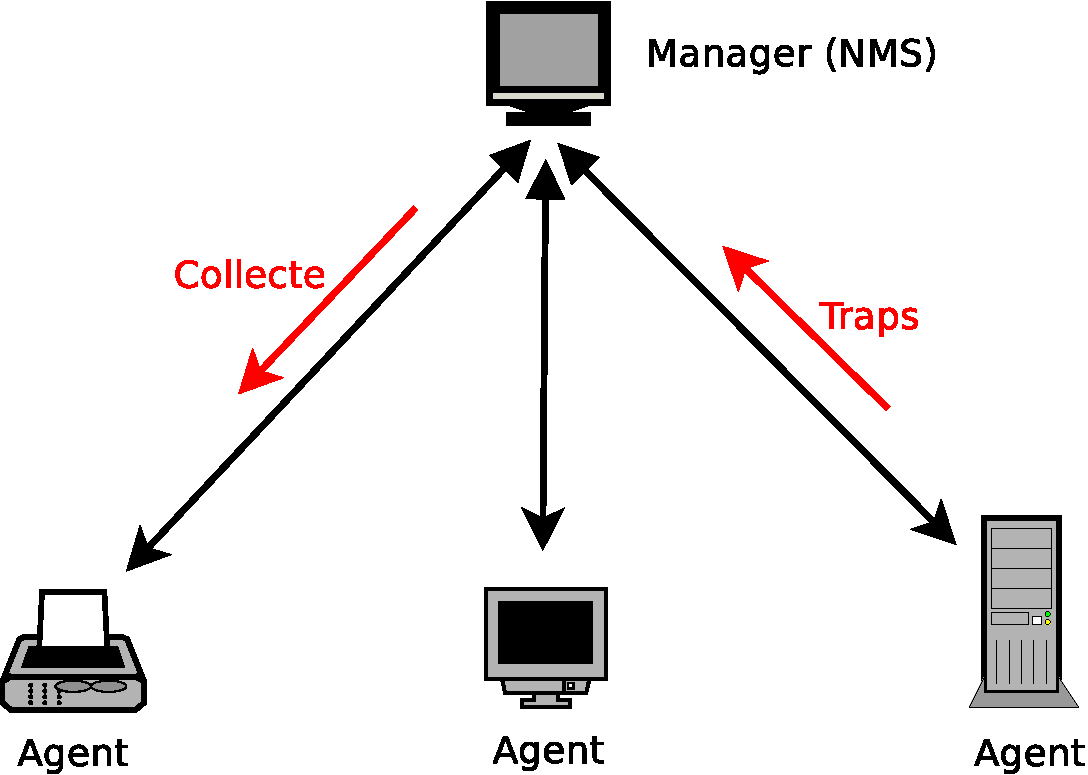
\includegraphics[scale=0.4]{images/snmp_principe.pdf}
     \caption{Mode de fonctionnement de SNMP. \label {fig:snmp}} 
    \end{center}
   \end{figure} 

\begin{itemize}
\item Fonctionne de manière asymétrique:  \emph{\gls*{agent}} et  \emph{\gls*{manager}} (\gls*{rfc} 1157).
\item Utilise des opérations en écriture (\texttt{set}) et en lecture (\texttt{get}).
\item Utilise \texttt{UDP} et le  \emph{\gls*{ber}} pour le transport.
\item Introduit le concept de  \emph{\gls*{mib}} (RCF 1213).
\item Identifie chaque \texttt{MIB} par son  \emph{\gls*{oid}}. 
\end{itemize}



Le présent mémoire porte  de manière générale sur l'implémentation en python de la découverte des équipements d'un réseau d'une organisation en utilisant \emph{\gls*{snmp}}. Cette découverte automatique des équipements du réseau servira de source d'importation des informations sur les équipements du réseau dans une solution libre de supervision: le \emph{\gls*{nav}}.

Le présent document se résume à notre apport pour l'\emph{initialisation automatique de la base de données} du \emph{\gls*{nav}}. Il est composé de deux chapitres:

\paragraph{Présentation théorique de la solution\\}

Le premier chapitre présente brièvement le \emph{\gls*{nav}}. \emph{\gls*{nav}} intègre bien d'autres solutions libres dont les plus importants sont Cricket, PostgreSQL, OpenStreeMap. Ce chapitre se termine sur le présentation de quelques limites du NAV disponible sur la feuille de route du projet. En particulier, l'accent est mis sur la fonctionnalité de l'\emph{autodiscovery-wizard}. Cette fonctionnalité permettra de fournir de manière automatique au NAV la base de données des équipements du réseau. Un début d'implémentation de cette fonctionnalité est donnée dans le cinquième chapitre.

\paragraph{Initialisation automatique de la base de données\\}
Le dernier chapitre constitue notre apport pour l'implémentation de l'\emph{autodiscovery-wizard}. Cette implémentation permet l'\emph{initialisation automatique de la base de données} du NAV. Plus besoin d'ajouter un à un les équipements du réseau ou bien de les lister soi-même dans un fichier. Notre solution en s'inspirant des études en matière de découverte de réseau sur la base de \emph{SNMP} permet de découvrir tous les équipements du réseau et de créer un fichier prêt pour importation dans la base de données du NAV. Après une présentation des algorithmes, l'implémentation en code python est expliquée, suivie des tests et résultats dans un environnement virtuel grâce à  \emph{\gls*{netkit}}.

